%!TEX root = ../konzeptpapier.tex
%!TEX spellcheck = de_DE
% Hauptmenuepunkt

%Hier der Inhalt von Überschrift 2 mit einem Beispielbild // und \citep[nach][12\psq]{ley2004soz} einem Literaturverweis
\begin{figure}[hbtp]
  \centering
  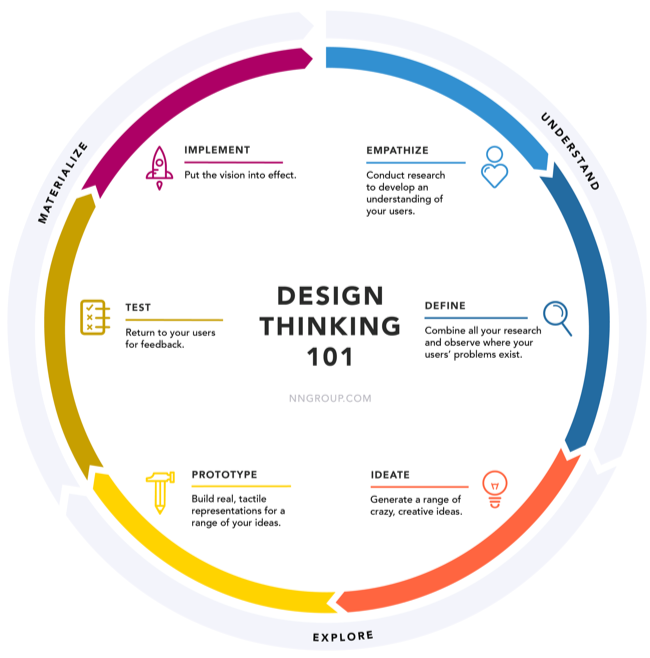
\includegraphics[width=0.85\textwidth]{res/design_thinking.png}
  \caption{Design Thinking 101 \citep[Quelle:][]{designthinking}}
  \label{fig:exintink}
\end{figure}
% label brauch man für verlinkungen, also in diesem fall unnötig
%\label{sec:refUeb1}

\section{EMPATHIZE}\label{EMPATHIZE}
\subsection{Beschreibung des Projektumfeldes}\label{Beschreibung des Projektumfeldes}
Beschreiben Sie unter diesem Punkt kurz das Umfeld (Ihr Unternehmen/ ihre Einrichtung/ Institution/ Verein) indem das Multimediaprodukt eingesetzt werden soll.
Welche Besonderheiten sind dort evtl. anzutreffen?
Gibt es Dinge, die man bei der Gestaltung eines Multimediaproduktes besonders beachten muss?

\subsection{Beschreibung der Zielgruppe}\label{Beschreibung der Zielgruppe}
Hier sollen Sie Ihre Zielgruppe beschreiben.
Welche Altersgruppe umfasst ihre Zielgruppe?
Liegen Einschränkungen vor?
Besondere Interessen oder Ansprüche?
Usw


\section{DEFINE}\label{DEFINE}


\subsection{Befragung von potentiellen Nutzern und/oder Kollegen}\label{Befragung von potentiellen Nutzern und/oder Kollegen}
Stellen Sie bitte folgende Fragen an Probanden Ihrer Zielgruppe/ oder falls diese nicht erreichbar sind Ihren Kollegen:

Fällt Ihnen spontan ein digitales Produkt/ Anwendung ein, die Sie ich im {Projektumfeld} wünschen würden?

Welche Abläufe/ Strukturen/ organisatorische Regelungen könnten in Ihrer Meinung nach (im Projektumfeld) verbessert werden?

Welche Ausgabemedien (Tablet, Smartphone, …) nutzen Sie am liebsten?

Kennen Sie eine digitale App/ Anwendung, die Sie sich gerne auch im Kontext {Ihres Projektumfeldes} vorstellen können?

(Gerne können Sie auch weitere Fragen formulieren, die Sie an die Probanden stellen und die Ihnen Inspirationen liefern können. )


\subsection{Ergebnisse der Befragung}\label{Ergebnisse der Befragung}
Stellen Sie hier bitte kurz die Ergebnisse der Befragung dar.

\subsection{Projektziel}\label{Projektziel}
Leiten Sie aus den Ergebnissen der Befragung ein Projektziel ab, welches Sie kurz formulieren

% Seitenumbruch
% \newpage

\section{IDEATE}\label{IDEATE}


\subsection{Produktidee (zur Lösung des Projektziels)}\label{Produktidee (zur Lösung des Projektziels) }
Entwickeln Sie eine Produktidee, diese Sie gerne als Prototyp als Lösungsansatz für das Projektziel umsetzen möchten.

\section{PROTOTYPE}\label{PROTOTYPE}

\subsection{Geplantes Ausgabemedium}\label{Geplantes Ausgabemedium}
Welches Ausgabemedium wollen Sie gerne für Ihren Prototypen nutzen? Mit kurzer Begründung bitte. Beachten Sie dazu bitte sowohl die Ergebnisse Ihrer Benutzerbefragung als auch die Voraussetzungen der Projektumgebung.

\subsection{Geplanter Medieneinsatz}\label{Geplanter Medieneinsatz}
Welche Medien (Audio/ Video/ Bild/ …) planen Sie einzusetzen?


